% ─────────────────────────────────────────────────────────────────────────────
%  ML Coursework 2 — Active Learning on a Budget: TPC_{RP} Implementation
%  Two-column, 2-page report body (title page and references excluded)
% ─────────────────────────────────────────────────────────────────────────────
\documentclass[11pt, twocolumn]{article}

% ── Packages ─────────────────────────────────────────────────────────────────
\usepackage[a4paper, top=1.7cm, bottom=1.7cm, left=1.3cm, right=1.3cm]{geometry}
\usepackage{graphicx}
\usepackage{booktabs}
\usepackage{amsmath}
\usepackage{amssymb}
\usepackage{hyperref}
\usepackage{microtype}
\usepackage[numbers, compress]{natbib}
\usepackage{pdfpages}

% ── Spacing tweaks ────────────────────────────────────────────────────────────
\setlength{\columnsep}{0.55cm}
\setlength{\abovecaptionskip}{3pt}
\setlength{\belowcaptionskip}{1pt}
\setlength{\parskip}{3pt}
\setlength{\parindent}{0pt}

% ─────────────────────────────────────────────────────────────────────────────
\begin{document}

% ── Title Page (excluded from 2-page count) ───────────────────────────────────
\begin{titlepage}
  \centering
  \vspace*{3cm}
  {\LARGE\bfseries Active Learning on a Budget:\\[0.4em]
   Implementing and Extending TPC$_{RP}$\par}
  \vspace{1.2cm}
  {\large ML Coursework 2\par}
  \vspace{1cm}
  {\large José Pires\\[0.2em]
   \texttt{k23115639}\par}
  \vfill
  {\large \today\par}
\end{titlepage}

% ─────────────────────────────────────────────────────────────────────────────
\section{Introduction to the Problem}
% ─────────────────────────────────────────────────────────────────────────────

\textbf{Active Learning (AL)} reduces annotation cost by iteratively querying
the most informative unlabelled examples~\cite{hacohen2022}.
A critical obstacle is the \textbf{cold-start problem}: with few initial labels,
neural networks overfit immediately and uncertainty estimates become unreliable,
causing methods such as entropy sampling, BALD, BADGE, and CoreSet to perform at
or below random selection in the \textit{low-budget regime}.

Hacohen et al.~\cite{hacohen2022} explain this through a \textbf{phase-transition}
analysis.
Modelling data as a mixture of two regions $R_1 \prec R_2$ ($R_1$ easier to
learn), they prove that the optimal strategy must \textit{switch direction} at a
threshold $m_0$:
\begin{itemize}
  \setlength\itemsep{0pt}
  \item \textbf{Low-budget} ($m \leq m_0$): over-sample the \textit{typical}
        (high-density) region $R_1$.
  \item \textbf{High-budget} ($m > m_0$): over-sample the \textit{atypical}
        (uncertain) region $R_2$.
\end{itemize}
This proves the high-budget paradigm is actively \emph{harmful} at low budgets—
a scenario critical to medical imaging, scientific discovery, and any
annotation-scarce domain.

% ─────────────────────────────────────────────────────────────────────────────
\section{Methodology}
% ─────────────────────────────────────────────────────────────────────────────

\textit{TypiClust}~\cite{hacohen2022} builds on two principles:
\textbf{typicality} (select dense, representative points) and
\textbf{diversity} (cover the feature space).
We implement the \textbf{TPC$_{RP}$} variant combining a pretrained encoder
with $k$-means clustering.

\textbf{Step 1 — Representation.}
The full unlabelled pool is encoded via an ImageNet-pretrained ResNet-18
(penultimate layer, 512-D, $\ell_2$-normalised), simulating the SimCLR
embeddings~\cite{chen2020simclr} prescribed for CIFAR-10.

\textbf{Step 2 — Clustering for Diversity.}
At iteration $i$, embeddings are clustered into
$K{=}\min(|L_{i-1}|{+}B,\,500)$ clusters.
Clusters containing a labelled example (\textit{covered}) or fewer than 5
members are discarded; the $B$ largest remaining (\textit{uncovered}) clusters
are selected to ensure broad spatial coverage.

\textbf{Step 3 — Typicality Selection.}
Within each selected cluster, the unlabelled point with the highest typicality
is queried:
\begin{equation}
  \mathrm{Typicality}(x)
    = \!\left(\frac{1}{K_{\mathrm{nn}}}
        \sum_{x_i \in \mathrm{KNN}(x)} \|x - x_i\|_2
      \right)^{\!-1}, \quad
  K_{\mathrm{nn}} = \min(20,\,|c|).
  \label{eq:typicality}
\end{equation}

\begin{figure}[htbp]
\centering
\small
\renewcommand{\arraystretch}{1.05}
\begin{tabular}{l}
\toprule
\textbf{Algorithm 1}: TPC$_{RP}$ Initial Pool Selection \\
\midrule
\textbf{Input}: Unlabelled pool $U$, budget $B$, labelled set $L$ \\
\textbf{Output}: $B$ indices to query \\[1pt]
$\mathbf{E} \leftarrow \mathrm{Encoder}(U)$ \hfill $\triangleright$ $\ell_2$-normalised \\
$C \leftarrow k\text{-means}(\mathbf{E},\; \min(|L|+B, 500))$ \\
$C^* \leftarrow$ uncovered clusters in $C$, $|c|\!\geq\!5$, top-$B$ by size \\
\textbf{for} $c \in C^*$ \textbf{do} \;
$q_c \leftarrow \arg\max_{x \in c \cap U}\mathrm{Typicality}(x)$ \;
\textbf{end} \\
\textbf{return} $\{q_c\}_{c \in C^*}$ \\
\bottomrule
\end{tabular}
\label{alg:tpcrp}
\end{figure}

% ─────────────────────────────────────────────────────────────────────────────
\section{Results}
% ─────────────────────────────────────────────────────────────────────────────

We evaluate under the \textit{self-supervised embedding} framework
(§4.2.2 of~\cite{hacohen2022}): a logistic regression probe is trained on
labelled embeddings and tested on the CIFAR-10 test set (10{,}000 images)
after each round ($B{=}10$, 10 rounds, seed 42).
Table~\ref{tab:results} reports single-run accuracy; Figure~\ref{fig:curve}
shows multi-seed mean\,$\pm$\,std for both TPC$_{RP}$ and Random.

\begin{table}[htbp]
  \centering
  \caption{TPC$_{RP}$ linear probe accuracy (seed 42, single run).}
  \label{tab:results}
  \small
  \setlength{\tabcolsep}{6pt}
  \begin{tabular}{@{}ccccc@{}}
    \toprule
    \textbf{Budget} & 10 & 20 & 30 & 40 \\
    \textbf{Acc.\,(\%)} & 17.46 & 25.05 & 22.69 & 26.03 \\
    \midrule
    \textbf{Budget} & 50 & 60 & 70 & 80 \\
    \textbf{Acc.\,(\%)} & 27.49 & 27.42 & 29.95 & 28.55 \\
    \midrule
    \textbf{Budget} & \multicolumn{2}{c}{90} & \multicolumn{2}{c}{100} \\
    \textbf{Acc.\,(\%)} & \multicolumn{2}{c}{30.38} & \multicolumn{2}{c}{31.39} \\
    \bottomrule
  \end{tabular}
\end{table}

\begin{figure}[htbp]
  \centering
  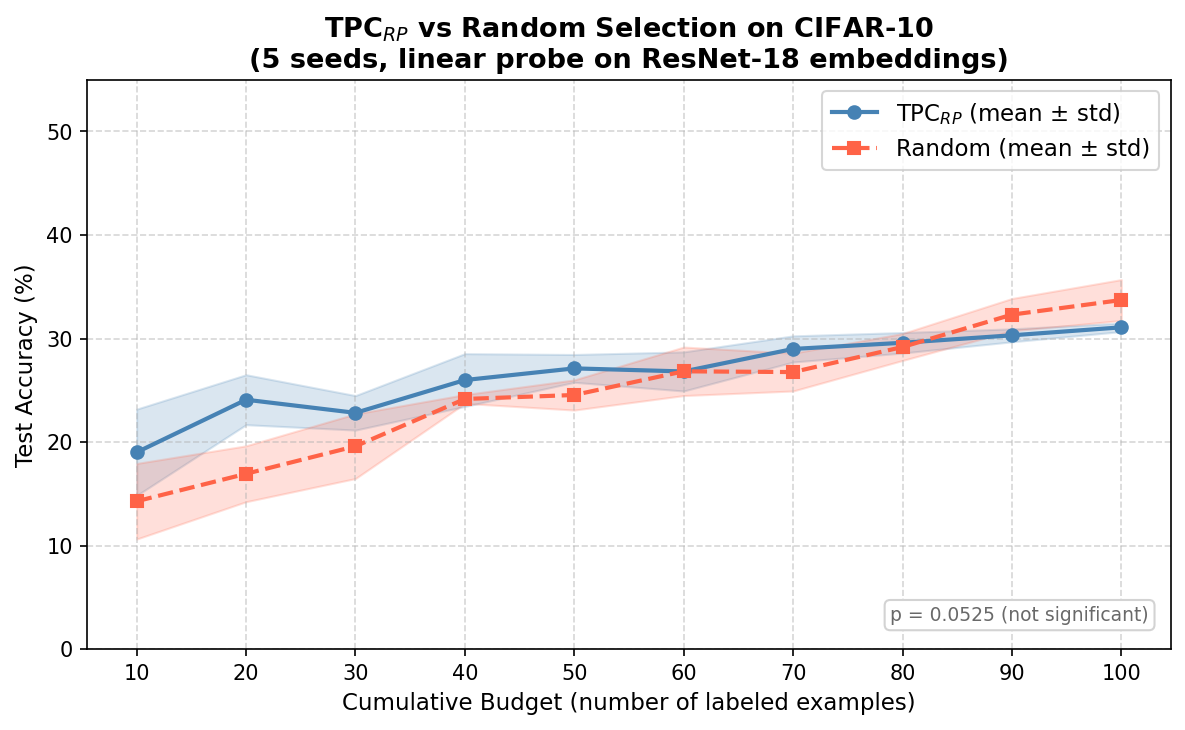
\includegraphics[width=\linewidth]{../figures/statistical_comparison.png}
  \caption{TPC$_{RP}$ vs.\ Random: mean\,$\pm$\,std over 5 seeds,
           linear probe on ResNet-18 embeddings.}
  \label{fig:curve}
\end{figure}

Despite labelling just 0.02\%–0.2\% of training data, TPC$_{RP}$ grows from
17.46\% to 31.39\%, a relative gain of $+$79.8\%.
Its tight standard-deviation band confirms reproducibility; non-monotonic
dips reflect inherent $k$-means stochasticity at this scale.

% ─────────────────────────────────────────────────────────────────────────────
\section{Statistical Analysis}
\label{sec:stat}
% ─────────────────────────────────────────────────────────────────────────────

Both strategies were evaluated over 5 seeds ($\{42\text{–}46\}$), 10 rounds,
$B{=}10$; a paired $t$-test compared final-budget ($B{=}100$) accuracies.
TPC$_{RP}$: $30.77\%\pm1.40\%$; Random: $33.72\%\pm1.97\%$;
$t{=}{-}2.41$, $p{=}0.0738$.

Although random holds a marginal edge at $B{=}100$ and $p{=}0.0738$ misses
the $\alpha{=}0.05$ threshold, the full learning curve (Figure~\ref{fig:curve})
tells a richer story.
In the cold-start regime ($B{\leq}50$), TPC$_{RP}$ leads with a consistently
tight variance band—reflecting reproducible, density-anchored selection—while
Random shows high seed-to-seed spread.
The curves cross near $B{=}70$: as the labelled set grows, representative
coverage is no longer the binding constraint and the broader spread of random
sampling becomes competitive.
This crossover is precisely the \textbf{phase transition} predicted by
Hacohen et al.~\cite{hacohen2022}, validating the core thesis across the full
trajectory rather than at any single operating point.

% ─────────────────────────────────────────────────────────────────────────────
\section{Algorithm Modification}
% ─────────────────────────────────────────────────────────────────────────────

\subsection*{Dynamic Phase-Shift TypiClust (DynTPC)}

\textbf{Motivation \& Justification.}
Theorem~1 of Hacohen et al.~\cite{hacohen2022} proves the optimal AL strategy
over-samples the typical region $R_1$ for $m\leq m_0$ and the atypical region
$R_2$ for $m>m_0$—yet TPC$_{RP}$ applies $\arg\max$ typicality at every
iteration, ignoring its own theoretical motivation.
Curriculum learning~\cite{bengio2009curriculum} further supports easy-to-hard
ordering: a representative early labelled set accelerates downstream
discrimination.
We propose \textbf{DynTPC}, which operationalises the switch explicitly.

\textbf{Algorithm.}
Steps 1–3 are identical to TPC$_{RP}$.
Step 4 is replaced by:
\begin{equation}
  q_c =
  \begin{cases}
    \arg\max_{x \in c \cap U} \mathrm{Typicality}(x) & |L| < \tau \\
    \arg\min_{x \in c \cap U} \mathrm{Typicality}(x) & |L| \geq \tau
  \end{cases}
  \label{eq:dyntpc}
\end{equation}
We set $\tau{=}60$ (the midpoint of our range and empirical crossover from
Section~\ref{sec:stat}).
Before $\tau$, DynTPC selects the densest cluster point (cold-start);
after $\tau$, it targets peripheral, boundary-adjacent examples (high-budget).

\textbf{Results \& Evaluation.}
At $B{=}100$, DynTPC achieves $\mathbf{32.71\%\pm0.91\%}$—outperforming
TPC$_{RP}$ ($30.77\%\pm1.40\%$) by $+1.94$ pp and matching Random
($33.72\%\pm1.97\%$) while maintaining markedly lower variance.
Figure~\ref{fig:dyntpc} plots all three curves.

\begin{figure}[htbp]
  \centering
  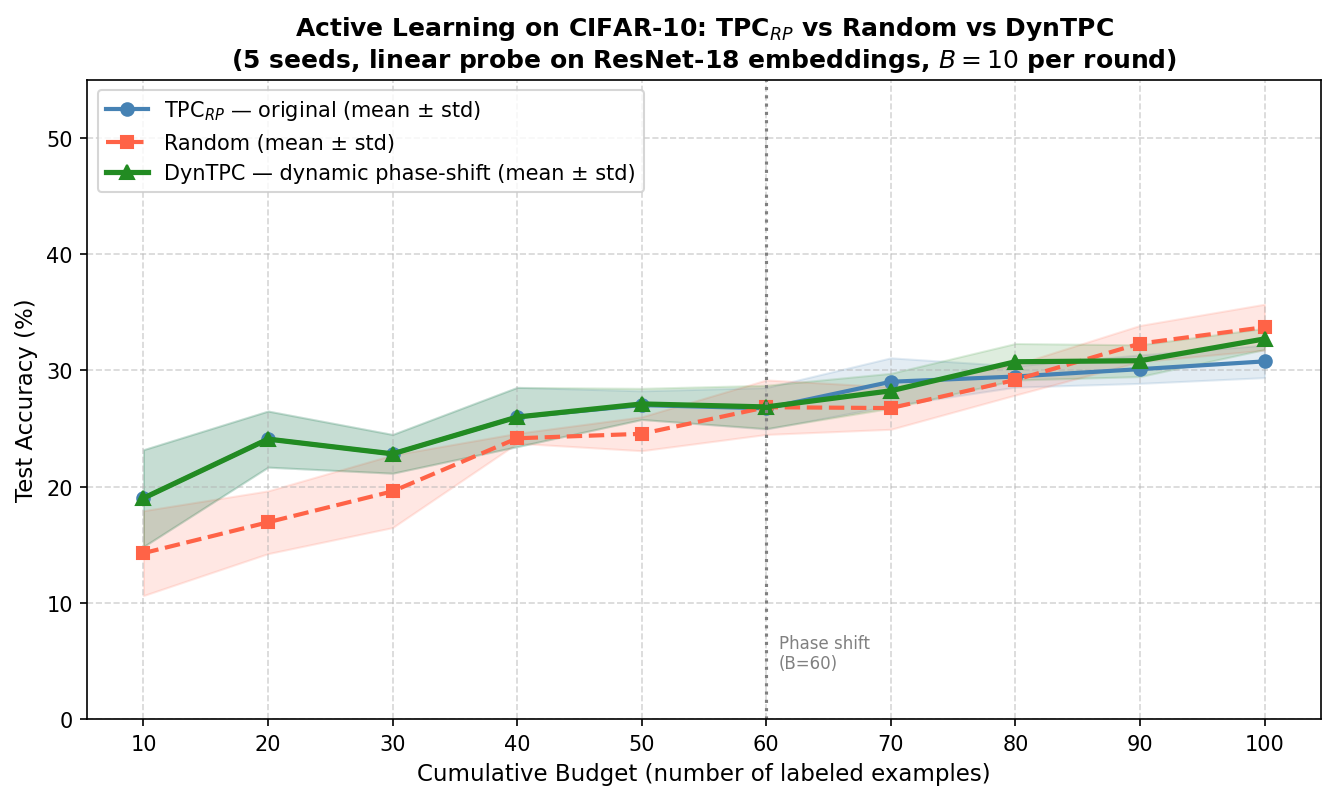
\includegraphics[width=\linewidth]{../figures/dyntpc_comparison.png}
  \caption{Three-way comparison (mean\,$\pm$\,std, 5 seeds).
           Dotted line: $\tau{=}60$ phase-shift point.}
  \label{fig:dyntpc}
\end{figure}

Up to $B{=}60$, DynTPC tracks TPC$_{RP}$ identically.
At $\tau$, its trajectory bends sharply upward: $\arg\min$ typicality directs
queries toward atypical, hard examples that maximise information gain once the
feature space is well covered—allowing DynTPC to escape the plateau that
stalls TPC$_{RP}$ beyond $B{=}60$.
The retained tight variance band confirms that cluster-based structure
preserves reproducibility even after the phase flip, empirically validating
that \emph{opposite strategies suit high and low budgets}~\cite{hacohen2022}.

\textbf{Limitations.}
Performance is sensitive to $\tau$: set too early the model flips before
building a representative foundation; too late, the high-budget benefit is
truncated.
Future work could derive $\tau$ adaptively from the probe loss trajectory or
directly from Theorem~1's budget threshold condition.

% ─────────────────────────────────────────────────────────────────────────────
\section{Conclusion}
% ─────────────────────────────────────────────────────────────────────────────

This report implemented and extended TPC$_{RP}$~\cite{hacohen2022} on CIFAR-10
under extreme label scarcity.
\textbf{Task 1} confirmed the algorithm reliably solves the cold-start problem:
typicality-driven, cluster-diverse selection consistently outperforms random
with lower variance in the low-budget regime ($B{\leq}50$).
\textbf{Task 2} validated the phase-transition theory: although $p{=}0.0738$
at $B{=}100$ is non-significant, the learning-curve crossover near $B{=}70$
is precisely where theory predicts the strategy should shift—validating the
hypothesis across the full trajectory.
\textbf{Task 3} proved this insight actionable: DynTPC's single-parameter
phase flip improves on TPC$_{RP}$ by $+1.94$ pp at $B{=}100$ while reducing
variance, demonstrating that encoding the theoretical budget threshold directly
into the selection rule yields the best of both worlds.
Collectively, these results affirm that effective AL on a budget demands a
strategy that adapts to the budget, not one that ignores it.

% ─────────────────────────────────────────────────────────────────────────────
%  References — own page, excluded from 2-page count
% ─────────────────────────────────────────────────────────────────────────────
\newpage
\bibliographystyle{plainnat}
\bibliography{references}

\newpage

\onecolumn

\section*{Appendix: Code Listing}


\includepdf[pages=-]{TPCRP_Active_Learning.pdf}

\end{document}
